\begin{frame}{Climbing Strings and Climbing Multistrings}
\begin{tikzpicture}[scaleall=1.0]
\pcuad{\textwidth}{\textheight}
\path(nw) 
    ++(0,-0.5) node(graphic1)[anchor=north west]{
        \nohyphens{Identify nearest \textcolor{red!80!black}{saddle points} to a free-energy minimum in feature space}
    }
    ++(0,-1) node(graphic1)[anchor=north west]{
        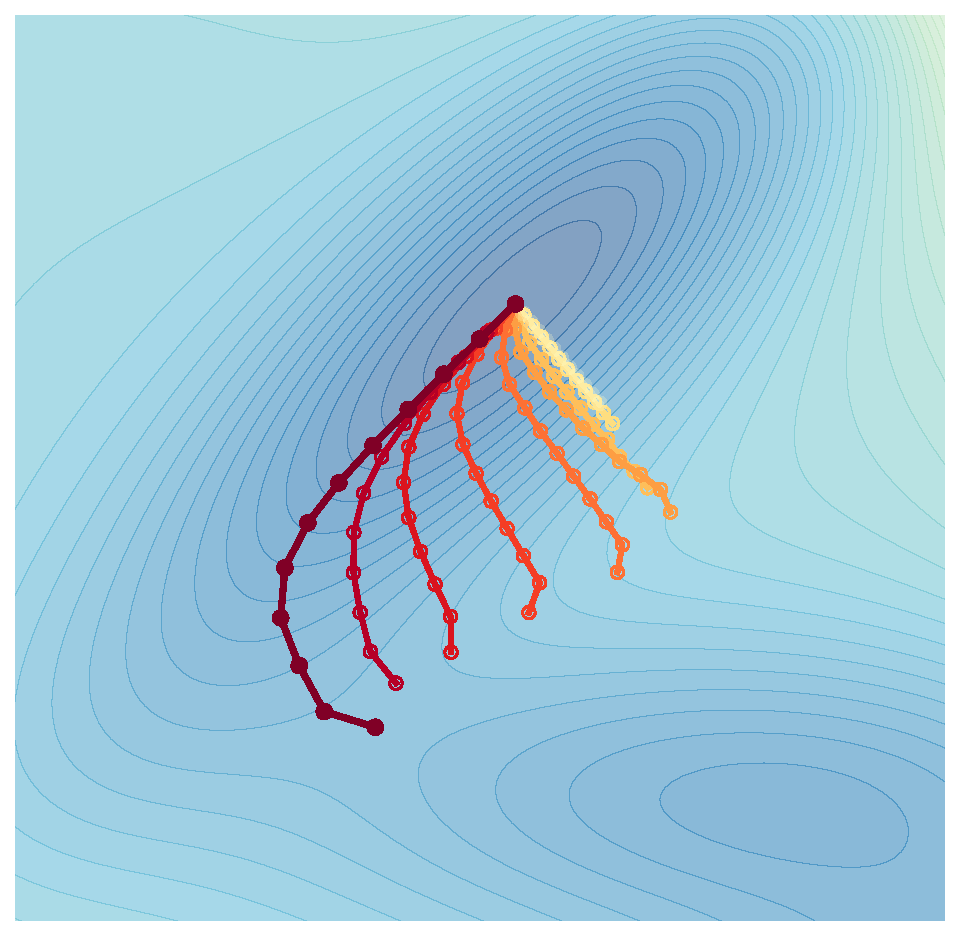
\includegraphics[width=0.5\textwidth]{csm.pdf}
    }
    ++(0.6\bbw,-0.5) node(eqns)[anchor=north west,text width=0.4\textwidth]{
        \nohyphens{Climbing image has force reversed along tangent $\hat{\taub}$}
    }
    ++(0,-1.5) node(lab1)[anchor=north west]{
        $\zb_N^\prime(t) = \zb_N(t) - \nu\ d\zb\cdot\hat{\taub}$
    }
    ++(0,-1) node(lab2)[anchor=north west]{
        $d\zb \equiv \zb_N(t) - \zb_N(t-\Delta t)$
    }
    ++(0,-1) node(lab3)[anchor=north west]{
        $\nu > 1$: friction parameter
    };
\end{tikzpicture}
\end{frame}